% This LaTeX document needs to be compiled with XeLaTeX.
\documentclass[10pt]{article}
\usepackage[utf8]{inputenc}
\usepackage{amsmath}
\usepackage{amsfonts}
\usepackage{amssymb}
\usepackage[version=4]{mhchem}
\usepackage{stmaryrd}
\usepackage{graphicx}
\usepackage[export]{adjustbox}
\graphicspath{ {./images/} }
\usepackage[fallback]{xeCJK}
\usepackage{polyglossia}
\usepackage{fontspec}
\setCJKmainfont{Noto Serif CJK TC}

\setmainlanguage{polish}
\setmainfont{CMU Serif}

\title{Instrukcja dla zdającego }

\author{}
\date{}


\begin{document}
\maketitle
\(\qquad\)

\begin{center}
\begin{tabular}{|l|l|l}
\hline
 & M A T E M A T Y K A - poziom podstawowy & 05 marca 2019 r \\
LSCDN &  &  \\
\hline
\end{tabular}
\end{center}

\begin{enumerate}
  \item Sprawdź, czy arkusz zawiera 16 stron (zadania 1-34). Ewentualne braki zgłoś przewodniczącemu zespołu nadzorującego egzamin.
  \item Rozwiązania zadań i odpowiedzi zamieść w miejscu na to przeznaczonym.
  \item Odpowiedzi do zadań zamkniętych (1-25) przenieś na kartę odpowiedzi, zaznaczając je w części karty przeznaczonej dla zdającego. Zamaluj pola do tego przeznaczone. Błędne zaznaczenie otocz kółkiem i zaznacz właściwe.
  \item Pamiętaj, że pominięcie argumentacji lub istotnych obliczeń w rozwiązaniu zadania otwartego (26-34) może spowodować, że za to rozwiązanie nie otrzymasz pełnej liczby punktów.
  \item Pisz czytelnie i używaj tylko długopisu lub pióra z czarnym tuszem lub atramentem.
  \item Nie używaj korektora, a błędne zapisy wyraźnie przekreśl.
  \item Pamiętaj, że zapisy w brudnopisie nie będą oceniane.
  \item Możesz korzystać z zestawu wzorów matematycznych, cyrkla i linijki oraz kalkulatora prostego.
  \item Na tej stronie oraz na karcie odpowiedzi wpisz swój kod lub nazwisko i imię - zgodnie z ustaleniami szkolnymi.
  \item Nie wpisuj żadnych znaków w części przeznaczonej dla egzaminatora.
\end{enumerate}

Czas pracy:\\
170 minut

Liczba punktów\\
do uzyskania: \(\mathbf{5 0}\)

\section*{Zadanie 1. (lp)}
Rozwiązaniem nierówności \((x-1)^{2} \geq x^{2}-1\) jest zbiór\\
A. \((-\infty ; 1)\)\\
B. \((1 ;+\infty)\)\\
C. \((-\infty ; 1>\)\\
D. \(<1 ;+\infty)\)

Zadanie 2. (lp)\\
Wyrażenie \(3 \log (x)+\log (y)-2 \log (z)\) jest równe\\
A. \(\log \frac{3 x y}{z^{2}}\)\\
B. \(\log \frac{x y^{2}}{z}\)\\
C. \(\log \frac{3 x y}{z^{2}}\)\\
D. \(\log \frac{x^{3} y}{z^{2}}\)

Zadanie 3. (lp)\\
Liczba o 10\% mniejsza od liczby, która jest o 20\% większa od liczby 1200 jest równa\\
A. 1340\\
B. 1296\\
C. 1440\\
D. 1080

Zadanie 4. (lp)\\
Suma liczby odwrotnej do \(\frac{3}{x+1}\) i przeciwnej do \(\frac{1-2 x}{15}\) jest równa\\
A. \(\frac{7 x+4}{15}\)\\
B. \(\frac{x+7}{15}\)\\
C. \(\frac{4 x+7}{15}\)\\
D. \(\frac{7 x-4}{15}\)

\section*{Zadanie 5. (lp)}
Punkt o współrzędnych \(\left(\frac{1}{2} ;-\frac{1}{2}\right)\) należy do wykresu funkcji logarytmicznej opisanej wzorem\\
A. \(f(x)=\log _{2} x\)\\
B. \(f(x)=\log _{\frac{1}{2}} x\)\\
C. \(f(x)=\log _{4} x\)\\
D. \(f(x)=\log _{\frac{1}{4}} x\)

Zadanie 6. (lp)\\
Jeżeli wiadomo, że punkt \(P=(3 ; 4)\) należy do wykresu funkcji \(f(x)=2^{x}+m\), to\\
A. \(m=-2\)\\
B. \(m=-4\)\\
C. \(m=4\)\\
D. \(m=2\)

\section*{Zadanie 7. (lp)}
Rozwiązaniem równania \(\frac{2 x-4}{x+4}=3(x \neq-4)\) jest liczba\\
A. -18\\
B. -16\\
C. 16\\
D. 18

Zadanie 8. (lp)\\
Jeżeli argument funkcji \(f(x)=4 x-1\) wzrośnie o 5 , to wartość funkcji wzrośnie o\\
A. 18\\
B. 19\\
C. 20\\
D. 21

Zadanie 9. (1p)\\
W układzie współrzędnych dane są punkty \(A=(x ; 6), B=(6 ;-4)\) oraz \(M=(2 ; y)\). Jeżeli punkt \(M\) jest środkiem odcinka \(A B\), to\\
A. \(x=2, y=-1\)\\
B. \(x=-2, y=1\)\\
C. \(x=-2, y=3\)\\
D. \(x=2, y=3\)

BRUDNOPIS (nie podlega ocenie)

\section*{Zadanie 10. (lp)}
Jeśli na rysunku przedstawiony jest wykres funkcji \(\mathrm{f}(\mathrm{x})\), to dziedziną funkcji \(g(x)=f(x+2)\) jest zbiór\\
A. \(\langle-2 ; 5\rangle\)\\
B. \(\langle-1 ; 4\rangle\)\\
C. \(\langle-5 ; 0\rangle\)\\
D. \(\langle-7 ; 1\rangle\)\\
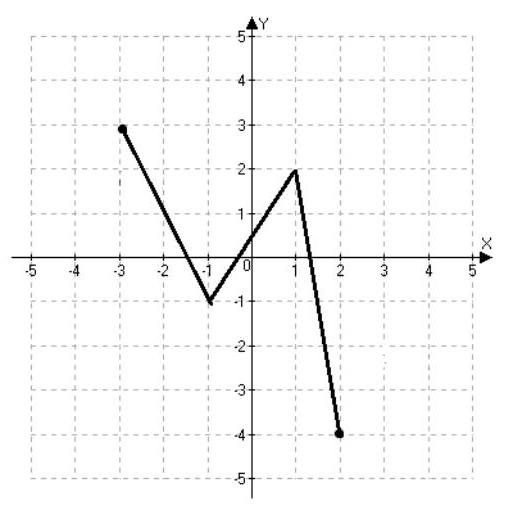
\includegraphics[max width=\textwidth, center]{2024_11_21_90ea54b753259b37713ag-04(1)}

Zadanie 11. (lp)\\
Najmniejszą liczbą całkowitą należącą do dziedziny funkcji \(f(x)=\sqrt{3 x-7}\) jest liczba\\
A. -3\\
B. -2\\
C. 2\\
D. 3

\section*{Zadanie 12. (lp)}
Jeśli wiadomo, że wierzchołek funkcji \(f(x)=3 x^{2}-4 k\) należy do prostej \(y=5\), to wartość liczbowa współczynnika \(\boldsymbol{k}\) jest równa\\
A. \(k=-\frac{5}{4}\)\\
B. \(k=-\frac{4}{5}\)\\
C. \(k=\frac{4}{5}\)\\
D. \(k=\frac{5}{4}\)

Zadanie 13. (lp)\\
Liczbę \(\frac{7}{11}\) przybliżono z dokładnością do \(10^{-1}\). Błąd względny tego przybliżenia jest równy\\
A. \(\frac{3}{70}\)\\
B. \(\frac{4}{70}\)\\
C. \(\frac{5}{70}\)\\
D. \(\frac{6}{70}\)

Zadanie 14. (lp)\\
Jeśli w ciągu arytmetycznym \(a_{2}=12\) i \(a_{6}=28\), to\\
A. \(a_{1}+a_{4}=30\)\\
B. \(a_{6}-a_{2}=18\)\\
C. \(a_{5}-a_{3}=10\)\\
D. \(a_{2}+a_{5}=36\)

Zadanie 15. (lp)\\
Jeśli \(\sin \alpha=\frac{1}{4}\), to długość przyprostokątnej \(\boldsymbol{a}\) danego trójkąta (patrz rysunek) jest równa\\
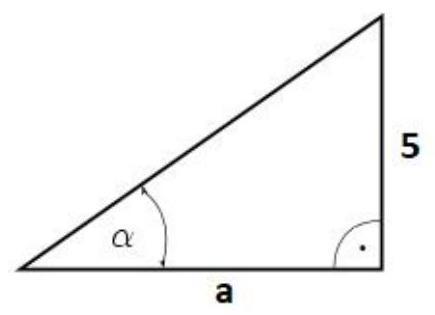
\includegraphics[max width=\textwidth, center]{2024_11_21_90ea54b753259b37713ag-04}\\
A. \(4 \sqrt{15}\)\\
B. \(5 \sqrt{15}\)\\
C. \(6 \sqrt{15}\)\\
D. \(7 \sqrt{15}\)

BRUDNOPIS (nie podlega ocenie)

Zadanie 16. (lp)\\
Tangens kąta ostrego \(\alpha\) jest równy 0,6 . Wówczas\\
A. \(\propto=40^{\circ}\)\\
B. \(\propto>40^{\circ}\)\\
C. \(\propto<40^{\circ}\)\\
D. \(\propto=30^{\circ}\)

Zadanie 17. (lp)\\
Miara kąta wpisanego jest o \(50^{\circ}\) mniejsza od miary kąta środkowego opartego na tym samym łuku okręgu. Zatem miara kąta wpisanego jest równa\\
A. \(40^{\circ}\)\\
B. \(50^{\circ}\)\\
C. \(60^{\circ}\)\\
D. \(70^{\circ}\)

Zadanie 18. (lp)\\
Pole równoległoboku o kącie ostrym równym \(60^{\circ}\) i długości boków wychodzących z wierzchołka tego kąta równych 6 i 8 jest równe\\
A. \(24 \sqrt{3}\)\\
B. \(24 \sqrt{2}\)\\
C. 24\\
D. \(16 \sqrt{3}\)

Zadanie 19. (lp) Funkcja liniowa \(f(x)=(2+3 k) x+3 k-2\) nie ma miejsc zerowych dla\\
A. \(k=-\frac{2}{3}\)\\
B. \(k=\frac{2}{3}\)\\
C. \(k=-\frac{1}{2}\)\\
D. \(k=\frac{1}{2}\)

Zadanie 20. (lp)\\
Jeśli suma n początkowych wyrazów ciągu arytmetycznego \(\left(a_{n}\right)\) określona jest wzorem \(S_{n}=4 n^{2}-n\), to wartość piątego wyrazu tego ciągu jest równa\\
A. 33\\
B. 35\\
C. 60\\
D. 95

Zadanie 21. (lp)\\
Dwa sąsiednie kąty równoległoboku różnią się o \(50^{\circ}\). Kąt ostry tego równoległoboku ma miarę\\
A. \(45^{\circ}\)\\
B. \(55^{\circ}\)\\
C. \(65^{\circ}\)\\
D. \(75^{\circ}\)

Zadanie 22. (lp)\\
Powierzchnia boczna walca po rozwinięciu jest kwadratem o polu \(16 \pi^{2}\). Objętość tego walca jest równa\\
A. \(8 \pi^{3}\)\\
B. \(16 \pi^{3}\)\\
C. \(8 \pi^{2}\)\\
D. \(16 \pi^{2}\)

Zadanie 23. (lp)\\
Promień podstawy stożka o objętości \(12 \pi\) i wysokości 4 jest równy\\
A. 1\\
B. 3\\
C. 6\\
D. 9

BRUDNOPIS (nie podlega ocenie)

Zadanie 24. (lp)\\
Miara kąta \(\propto\) (patrz rysunek obok) jest równa\\
A. \(45^{\circ}\)\\
B. \(50^{\circ}\)\\
C. \(55^{\circ}\)\\
D. \(60^{\circ}\)\\
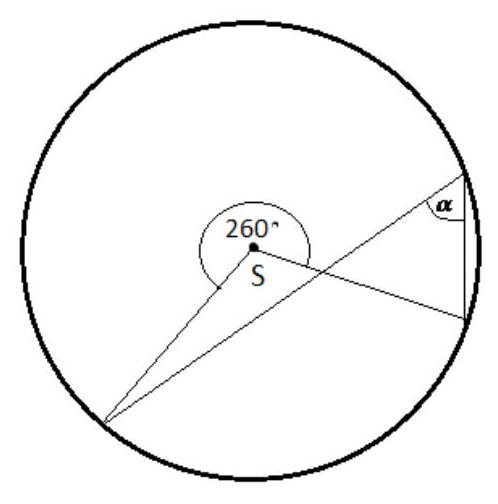
\includegraphics[max width=\textwidth, center]{2024_11_21_90ea54b753259b37713ag-08}

\section*{Zadanie 25. (lp)}
Ze zbioru kolejnych liczb naturalnych \(\{1,2,3, \ldots, 20\}\) losujemy jedną liczbę. Prawdopodobieństwo, że wylosujemy liczbę podzielną przez 3 jest równe\\
A. \(\frac{8}{20}\)\\
B. \(\frac{7}{20}\)\\
C. \(\frac{6}{20}\)\\
D. \(\frac{5}{20}\)

\section*{BRUDNOPIS (nie podlega ocenie)}
\section*{ZADANIA OTWARTE}
Rozwiazania zadań o numerach od 26 do 34 należy zapisać \(w\) wyznaczonych miejscach pod treściq zadania (pamiętaj o udzieleniu odpowiedzi)

Zadanie 26. (2p)\\
Rozwiąż nierówność \(-x(x-1) \leq-2\).

Zadanie 27. (2p)\\
Uzasadnij, że nie istnieją dwie liczby, których suma jest równa 4, a ich iloczyn jest równy 5.\\

\includegraphics[max width=\textwidth, center]{2024_11_21_90ea54b753259b37713ag-09(1)}

Zadanie 28. (2p)\\
W prostokącie ABCD punkt K jest środkiem boku BC, a punkt L środkiem boku DC. Wykaż, że pole trójkąta AKL jest równe sumie pól trójkątów ALD oraz KCL.\\
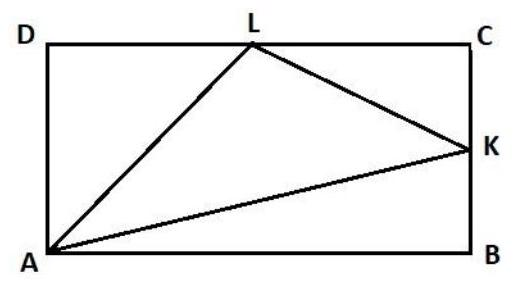
\includegraphics[max width=\textwidth, center]{2024_11_21_90ea54b753259b37713ag-09}

\section*{LUBELSKA PRÓBA PRZED MATURĄ 2019 - poziom podstawowy}
\section*{Zadanie 29. (2p)}
Dany jest trójkąt prostokątny o polu \(\frac{3 \sqrt{3}}{2}\) i kącie ostrym \(30^{\circ}\). Oblicz długości przyprostokątnych tego trójkąta.

\section*{Zadanie 30. (2p)}
Z punktu leżącego na okręgu o promieniu 5 poprowadzono dwie prostopadłe cięciwy. Różnica ich długości jest równa 2. Oblicz długości tych cięciw.\\

\includegraphics[max width=\textwidth, center]{2024_11_21_90ea54b753259b37713ag-10}

\section*{Zadanie 31. (2p)}
Dany jest trójmian kwadratowy \(f\) o współczynniku 3 przy najwyższej potędze \(x\). Wierzchołek paraboli będącej wykresem tego trójmianu ma współrzędne \(W=(5 ;-10)\). Wyznacz \(f(10)\).

\section*{LUBELSKA PRÓBA PRZED MATURĄ 2019 - poziom podstawowy}
Zadanie 32. (4p)\\
Przekątna graniastosłupa prawidłowego czworokątnego o długości 10 cm jest nachylona do płaszczyzny podstawy pod kątem \(\alpha=30^{\circ}\). Oblicz objętość tego graniastosłupa.

\section*{LUBELSKA PRÓBA PRZED MATURĄ 2019 - poziom podstawowy}
\section*{Zadanie 33. (4p)}
Ze zbioru \(\{1,2,3,4,5,6,7\}\) losujemy liczbę \(x\), a ze zbioru \(\{-7,-6,-5,-4,-3,-2,-1\}\) liczbę y. Oblicz prawdopodobieństwo tego, że \(x+y>2\).

\section*{LUBELSKA PRÓBA PRZED MATURĄ 2019 - poziom podstawowy}
\section*{Zadanie 34. (5p)}
Trzy liczby a, b, c tworzą ciąg arytmetyczny. Ich suma jest równa 15. Jeżeli pierwszą i trzecią pozostawimy bez zmian, a drugą pomniejszymy o jeden, to otrzymamy trzy kolejne wyrazy ciągu geometrycznego. Oblicz wyrazy ciągu arytmetycznego.

\section*{BRUDNOPIS (nie podlega ocenie)}
KARTA ODPOWIEDZI\\
KOD UCZNIA \(\square \square\)

Nazwisko iimię

Wypelnia piszący

\begin{center}
\begin{tabular}{|c|c|c|c|c|}
\hline
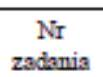
\includegraphics[max width=\textwidth]{2024_11_21_90ea54b753259b37713ag-16}
 & A & B & C & D \\
\hline
1. & ㅁ & ㅁ & ㅁ & ㅁ \\
\hline
2. & ㅁ & ㅁ & ㅁ & ㅁ \\
\hline
3. & ㅁ & ㅁ & ㅁ & ㅁ \\
\hline
4. & ㅁ & ㅁ & ㅁ & ㅁ \\
\hline
5. & ㅁ & ㅁ & ㅁ & ㅁ \\
\hline
6. & ㅁ & ㅁ & ㅁ & ㅁ \\
\hline
7. & 口 & ㅁ & ㅁ & ㅁ \\
\hline
8. & ㅁ & ㅁ & ㅁ & ㅁ \\
\hline
9. & 口 & ㅁ & ㅁ & ㅁ \\
\hline
10. & ㅁ & ㅁ & ㅁ & ㅁ \\
\hline
11. & ㅁ & ㅁ & ㅁ & ㅁ \\
\hline
12. & 口 & ㅁ & ㅁ & ㅁ \\
\hline
13. & - & ㅁ & ㅁ & ㅁ \\
\hline
14. & ㅁ & ㅁ & ㅁ & ㅁ \\
\hline
15. & ㅁ & ㅁ & ㅁ & ㅁ \\
\hline
16. & ㅁ & ㅁ & ㅁ & ㅁ \\
\hline
17. & ㅁ & ㅁ & ㅁ & ㅁ \\
\hline
18. & 口 & 口 & ㅁ & ㅁ \\
\hline
19. & ㅁ & ㅁ & ㅁ & ㅁ \\
\hline
20. & ㅁ & ㅁ & ㅁ & ㅁ \\
\hline
21. & 口 & ㅁ & ㅁ & ㅁ \\
\hline
22. & ㅁ & ㅁ & ㅁ & ㅁ \\
\hline
23. & ㅁ & ㅁ & ㅁ & ㅁ \\
\hline
24. & ㅁ & ㅁ & ㅁ & ㅁ \\
\hline
25. & ㅁ & ㅁ & ㅁ & ㅁ \\
\hline
\end{tabular}
\end{center}

Razem \(\square\)

\section*{Wypełnia sprawdzający}
\begin{center}
\begin{tabular}{|c|c|c|c|c|}
\hline
\( \begin{gathered} \mathrm{Nr} \\ \text { zadranis } \end{gathered} \) & X & 0 & 1 & 2 \\
\hline
26. & ㅁ & ㅁ & ㅁ & ㅁ \\
\hline
27. & ㅁ & ■ & ㅁ & ■ \\
\hline
28. & ㅁ & ■ & ㅁ & ■ \\
\hline
29. & ㅁ & ㅁ & ㅁ & ㅁ \\
\hline
30. & ㅁ & ■ & ㅁ & ■ \\
\hline
31. & ㅁ & ■ & ■ & ■ \\
\hline
\end{tabular}
\end{center}

Razem \(\square\)

\begin{center}
\begin{tabular}{|c|c|c|c|c|c|c|c|}
\hline
Nin & X & 0 & 1 & 2 & 3 & 4 & 5 \\
\hline
zadania & X & \(\square\) &  &  &  &  &  \\
\hline
32. & \(\square\) & \(\square\) & \(\square\) & \(\square\) & \(\square\) & \(\square\) &  \\
\hline
33. & \(\square\) & \(\square\) & \(\square\) & \(\square\) & \(\square\) & \(\square\) &  \\
\hline
34. & \(\square\) & \(\square\) & \(\square\) & \(\square\) & \(\square\) & \(\square\) & \(\square\) \\
\hline
\end{tabular}
\end{center}

Razem \(\square\)

\begin{center}
\begin{tabular}{|l|l|}
\hline
Suma punktów & Wynik w\% \\
\hline
 &  \\
 &  \\
\hline
\end{tabular}
\end{center}


\end{document}